\section{Other findings}
\label{sec:joleen}

	\subsection{Codeine --- to the tune of Jolene (Dolly Parton)}
		
		\begin{verse}
			\begin{centering}
			\note CODEINE \enote 
			 \vspace{0.3cm}
		
				Codeine, codeine, codeine, codeine!
				
				
				I'm begging of you take away my pain\\
				Codeine, codeine,codeine, codeine!\\
				Please just numb this feeling in my brain.
				
				
				As a powder you're beyond compare\\
				Effervescing when there's water there\\
				Your bubbles rising, bursting with a gleam
				
				
				In tablet form you taste so sweet\\
				Though I really shouldn't eat you neat\\
				But I cannot resist your lure codeine
				
				
				\emph{(chorus)}
				
				
				The constant ache within my bones\\
				The bruises which induce my moans\\
				You take it all away from me codeine.
				
				
				Every day and every night\\
				I cannot live without the sight\\
				or smell or taste or feel of you codeine.
				
				
				But my prescriptions running low\\
				Just fourteen packets left to go,\\
				Two sheets per pack right now, then let me see…
				
				
				There's eight of you sealed in a sheet\\
				That's 2-2-4 left for this week\\
				And then I'm on my own again codei … ne
				
			\end{centering}
		\end{verse}

\subsection{S1} Tetley and James 'Jimmy Dubz' Wilson went on a reconnaissance mission in \passage[cave]{S1} to find the origin of its freezing draught. The known end of the cave is an ascending boulder choke, which is incredibly difficult to dig. Over the years, piles of old tent poles have been left at this front, as successive explorers failed to progress any further. 

The motivation behind this cave is that it is within 110m from the eastern end of \passage{Hotline} in \passage{Migovec}, a freezing tube which had proved key to several early connections. Inside the cave, the pair also decided to have a look at a slightly deeper lead. Some further pushing by the Wilson brothers resulted in marginal progress over a tight rift, as well as the loss of the 2.5kg lump hammer. 

\subsection{Apple Crumble} Spurred on by the need to 'go left into blank mountain', Jimmy Dibz and I  traversed across the \passage{Povezava} aven on the \passage{TTT} route, gaining a large window above the shaft floor. The up-and-down rift passage quickly degenerated to a rabbit warren of tight, crumbly mud crawls with little draught. 

A small drop into a very immature streamway led to a bizarre cylindrical window into the roof the main \passage{TTT} route, downstream of \passage{Povezava} aven: an unfortunate connection. The trickle of water disappeared downstream in a small crack. It is my belief that the water reappears as the spout above \passage{Batmere}. It's just too bloody tight to follow! \name{Tanguy Racine}

\subsection{High and Dry} William French, Jimmy Dubz and I went back to the \passage{Hammerhead} area to inspect the undescended pitch beneath \passage{Dogfish}. After some intense gardening of the conglomerate layer at the pitch head, I sent Jimmy down first who shouted back `At least it's not dead'. 

Landing in a rift of sizeable dimensions, we found a P20 landing on precarious boulders and increasingly sketchy climbs under all this shattered rock mass. We called it \passage{High and Dry} as it was anything but, and surveyed out. At -501m it was my deepest point in \passage{Primadona} this year, and what a dead end it was! \name{Tanguy Racine}

\begin{pagefigure}
	\frame{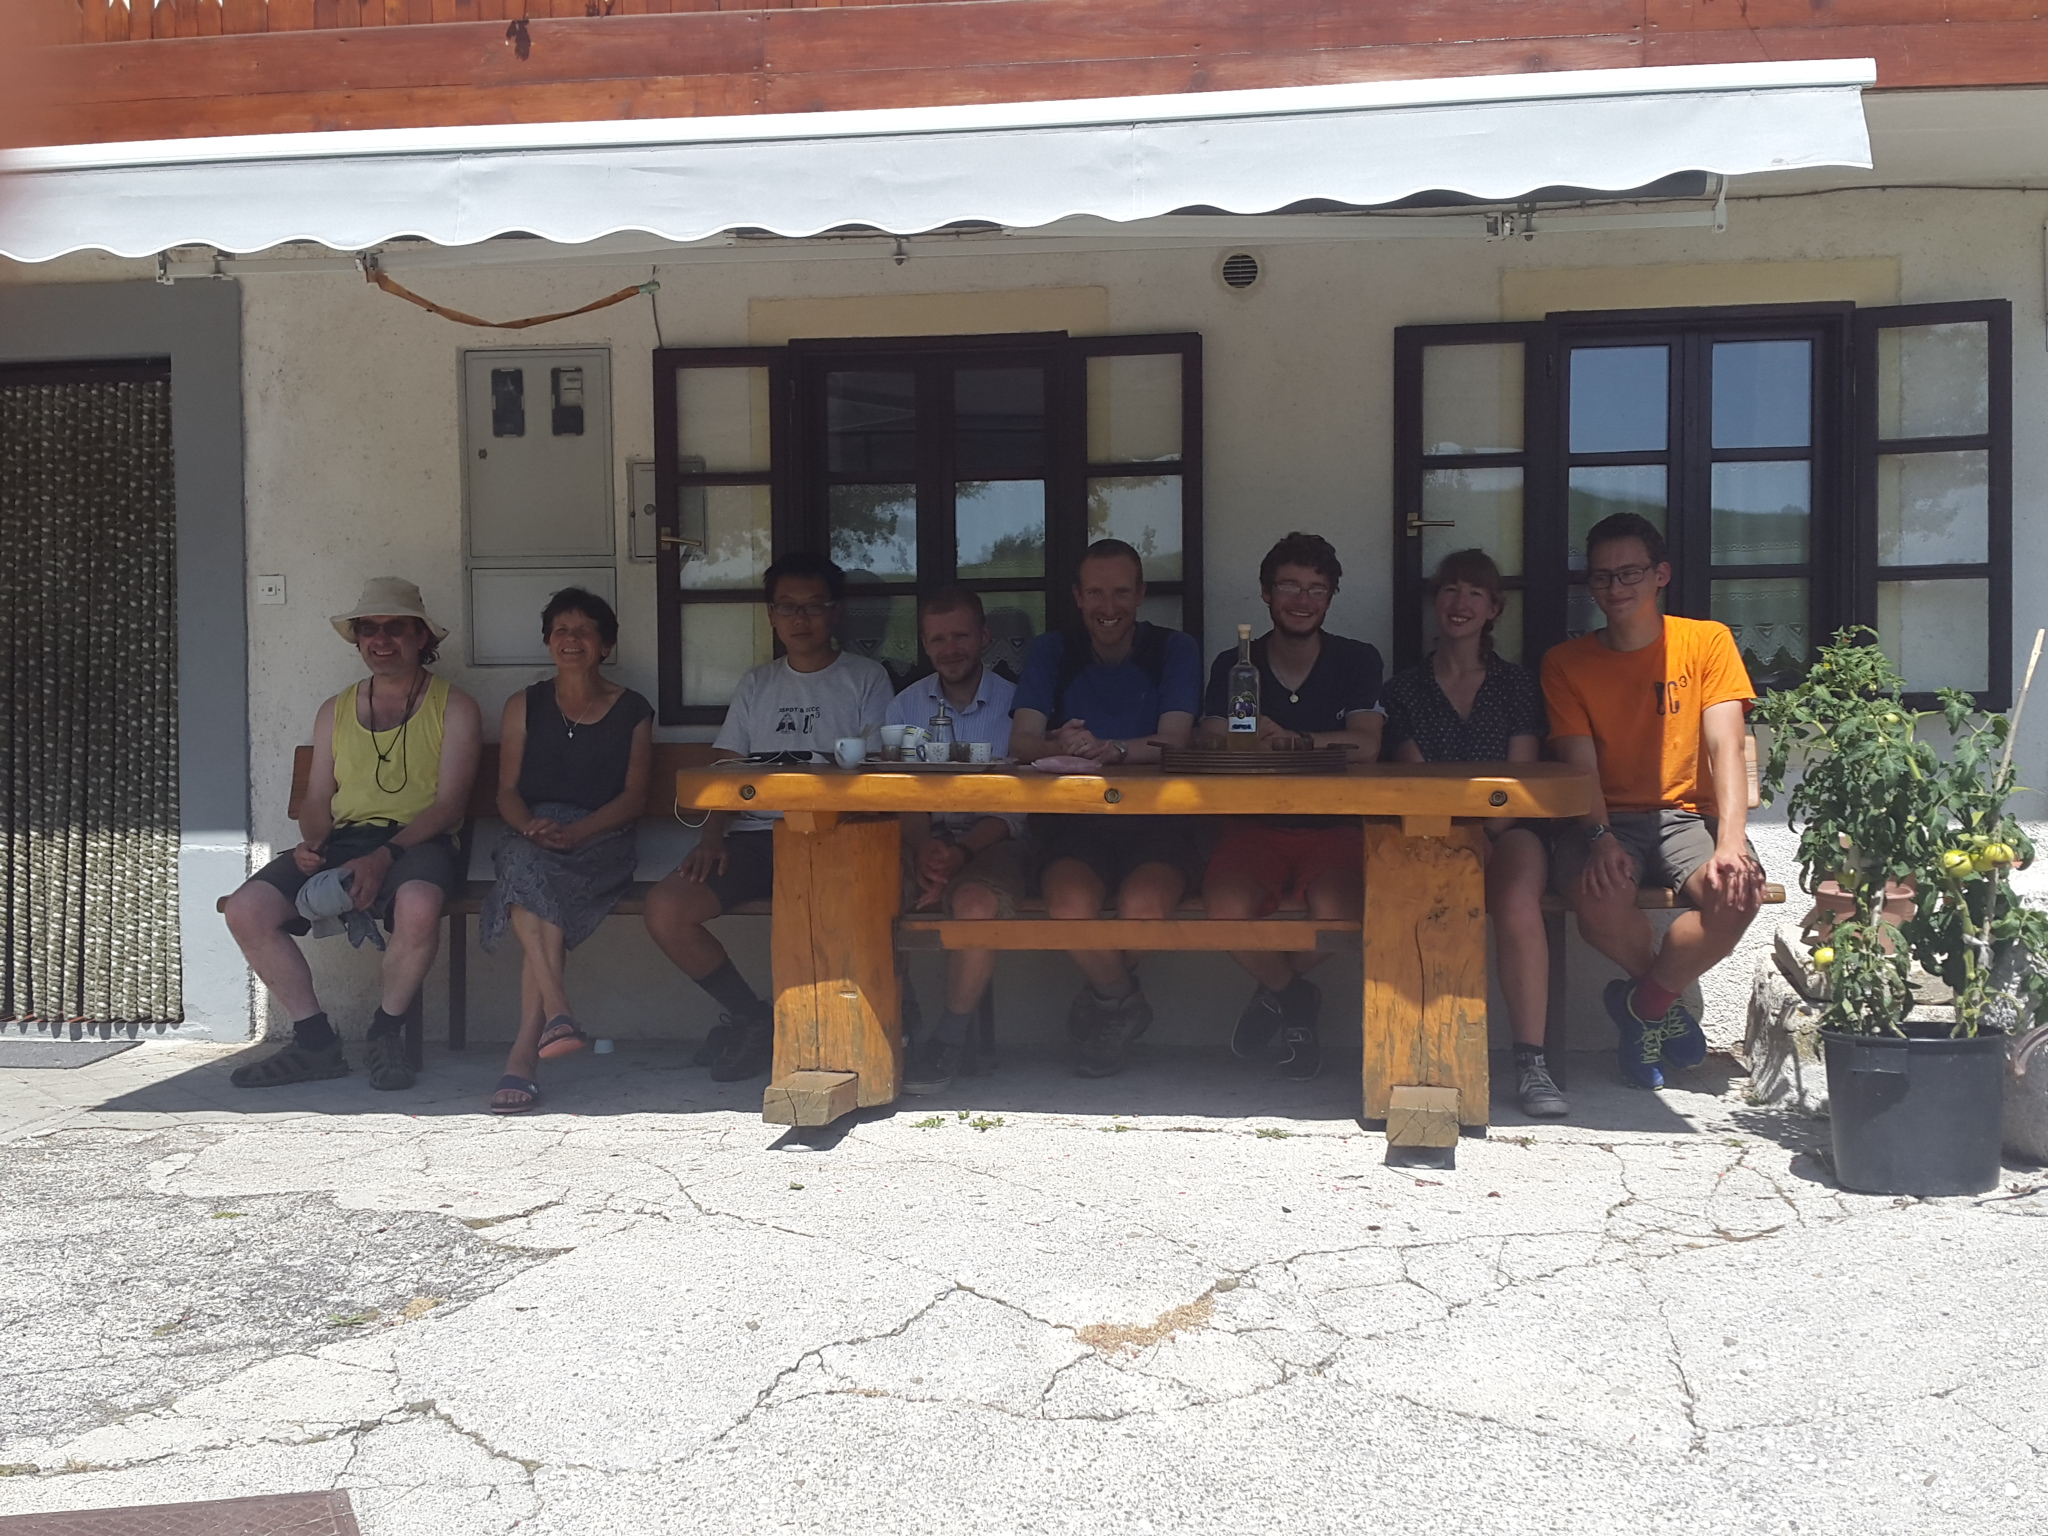
\includegraphics[width=\linewidth]{images/2017/other-finds-2017/end_of_expo_2017.jpg}}
	\caption{The team at the end of the \emph{\v{C}ez Rob} expedition \emph{from left to right} David Wilson, Slavica Koblu\v{c}ar, Larry Jiu Jiang, William French, Andy Jurd, Tanguy Racine, Kate Smith, David Wilson II \pic{Janet Cotter}}
	\label{fig:end expo 2017}
\end{pagefigure}
	
\numbertable{
							\begin{tabular}{llrrr}
    								\multicolumn{1}{l}{Sector} & Passage name & Survey length (m) & Stations & Average leg (m) \\ \midrule
    								\multicolumn{1}{l}{Alkatraz} & Testing the Waters & \_    & 22    & \_ \\ \midrule
   								 \multicolumn{1}{l}{\multirow{5}[0]{*}{Déjà Vu}} & Dogfish & 35.6  & 11    & 3.56 \\
          								& Hammerhead & 58.63 & 10    & 6.51 \\
          								& Hammerhead2 & 159.99 & 25    & 6.67 \\
									& Hammerhead3 & 22.72 & 6     & 4.54 \\
          								& High and Dry & 57.69 & 13    & 4.81 \\ \midrule
    								\multicolumn{1}{l}{\multirow{7}[0]{*}{Fenestrator}} & Alabaster & 113.61 & 27    & 4.37 \\
         							 & Battery Flattery & 63.42 & 12    & 5.77 \\
         							 & Fenestrator & 51.24 & 12    & 4.66 \\
         							 & Hallelujah & 34.46 & 11    & 3.45 \\
     							         & Plumber's Paradise & 107.67 & 26    & 4.31 \\
         						          & Sweet Baby Jesus & 105.17 & 24    & 4.57 \\
         							 & Union Passage of the Year Nominee & 32.16 & 14    & 2.47 \\ \midrule
    								\multicolumn{1}{l}{\multirow{6}[0]{*}{Karstaway}} & Electric Dreams & 151.6 & 26    & 6.06 \\
         							 & Entirely my fault & 78.54 & 20    & 4.13 \\
          							& More Like Welding & 87.37 & 17    & 5.46 \\
         							 & Stranglehold & 123.22 & 34    & 3.73 \\
         							 & The Atrium & 77.78 & 10    & 8.64 \\
         							 & What a Disappointment & 39.17 & 10    & 4.35 \\ \midrule
   							        \multicolumn{1}{l}{M16 entrance} & Death by 1000 blows & 17.32 & 11    & 1.73 \\ 							        \midrule
    								\multicolumn{1}{l}{\multirow{5}[0]{*}{Mandare}} & Apple Crumble & 97.62 & 27    & 3.75 \\
         							& Batmere & 66.33 & 13    & 5.53 \\
     								& Buckwheat resurvey & \_    & 9     & \_ \\
      							        & Mandare Resurvey & \_    & 8     & \_ \\
                          					& TTT\_resurvey & \_    & 48    & \_ \\ \midrule
   								\multicolumn{1}{l}{Smer0} & Jack of Hearts & 191.93 & 36    & 5.48 \\ \midrule
  								\multicolumn{1}{l}{Surface} & Gondolin & 113.08 & 16    & 7.54 \\ \midrule
          							&       &       &       &  \\

             							\textbf{Total} &       & \textbf{1886.32} &       &  \\
    							\end{tabular}}



	\begin{pagesurvey}
		\centering
		\frame{\includegraphics[height=\textheight]{"images/2017/other-finds-2017/2017plan".pdf}}
		\caption{2017 Plan Survey}
		\label{}
	\end{pagesurvey}

	\begin{pagesurvey}
		\centering
		\frame{\includegraphics[height=\textheight]{"images/2017/other-finds-2017/ee2017".pdf}}
		\caption{2017 Extended Elevation}
		\label{}
	\end{pagesurvey}
